%  \documentclass[oneside,11pt]{article}

% \input{preamble.tex}
% %%% HELPER CODE FOR DEALING WITH EXTERNAL REFERENCES
% \usepackage{xr}
% \makeatletter
% \newcommand*{\addFileDependency}[1]{
%   \typeout{(#1)}
%   \@addtofilelist{#1}
%   \IfFileExists{#1}{}{\typeout{No file #1.}}
% }
% \makeatother


% \newcommand*{\myexternaldocument}[1]{
%     \externaldocument{#1}
%     \addFileDependency{#1.tex}
%     \addFileDependency{#1.aux}
% }

% %\myexternaldocument{OA}

% %%%%%%%%%%%%%%%%%%%%%%%%%%%%%%%% DOCUMENT
% \begin{document}

%%%%%%%%%%%%%%%%%%%%%%%%%%%%%%%%%%%%%%%%%%%%%%%

% APPENDIX 
\setcounter{table}{0}
\setcounter{figure}{0}
\setcounter{section}{0}
\pagenumbering{gobble}


\begin{center}
	\LARGE Bargaining with (more) common priors in the field \\[0.5em]
	\Large{Appendix $-$ For Online Publication} \\[1em]
	\large \author{Joyce Sadka \and Enrique Seira  \and Christopher Woodruff}
\end{center}

\appendix
\pagenumbering{arabic}
\renewcommand\thefigure{OA-\arabic{figure}}
\renewcommand\thetable{OA-\arabic{table}}
\renewcommand*{\thepage}{OA - \arabic{page}}
\renewcommand\thesection{Appendix \Alph{section}.}
\renewcommand\thesubsection{\Alph{section}.\arabic{subsection}}

%\renewcommand{\cftparskip}{0em} % NOT NEEDED
\renewcommand\cftsecdotsep{\cftdotsep}
\renewcommand\cftsubsecdotsep{\cftnodots}
\renewcommand{\cftsecnumwidth}{6em}
 \renewcommand{\cftpnumalign}{r}
%\renewcommand{\cftsecleader}{\normalfont\cftdotfill{\cftsecdotsep}}


\renewcommand{\cftsecleader}{\cftdotfill{\cftsecdotsep}\hspace{1.8em}}
%\renewcommand{\cftsecpagefont}{20em}
%\renewcommand{\cftfignumwidth}{6em}
%\renewcommand{\cfttabnumwidth}{3.3em}

%\tableofcontents
\etocdepthtag.toc{mtappendix}
\etocsettagdepth{mtchapter}{none}
\etocsettagdepth{mtappendix}{subsection}

\setstretch{0.9}
%\renewcommand\contentsname{} % the empty name

\begingroup
\let\clearpage\relax
%\vspace{-1.5em} % the removed space. Set as appropriate
\tableofcontents
\endgroup


\newpage



\section{ -Robustness : Validation and falsification of the RD design}
\vspace{.2in}


\begin{figure}[H]
     \caption{RD plots (Control)}
    \label{rd_control}
\begin{center}
\begin{subfigure}{0.31\textwidth}
\caption{II vs I (Tenure)}
        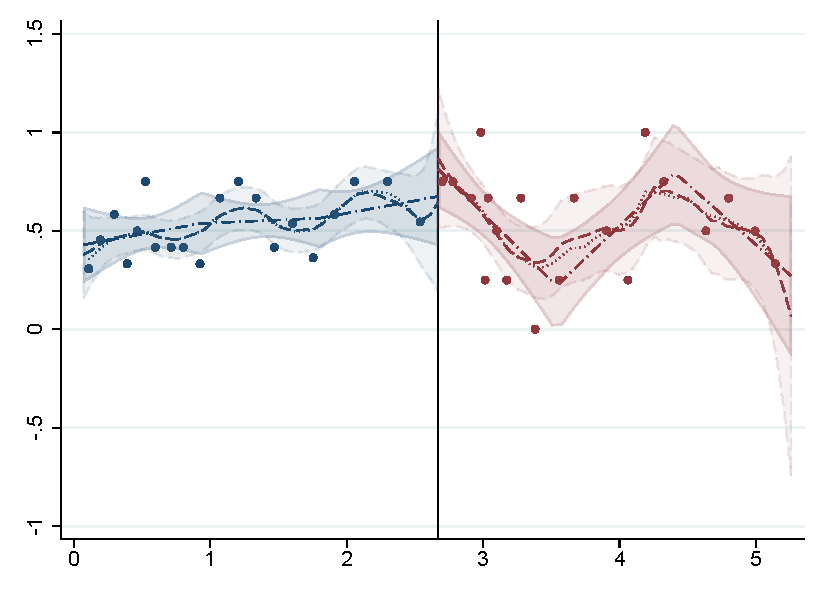
\includegraphics[width=\textwidth]{Figuras/rdplot_conflicto_arreglado_1_2_1.pdf}
    \end{subfigure}
    \begin{subfigure}{0.31\textwidth}
\caption{III vs IV (Tenure)}
        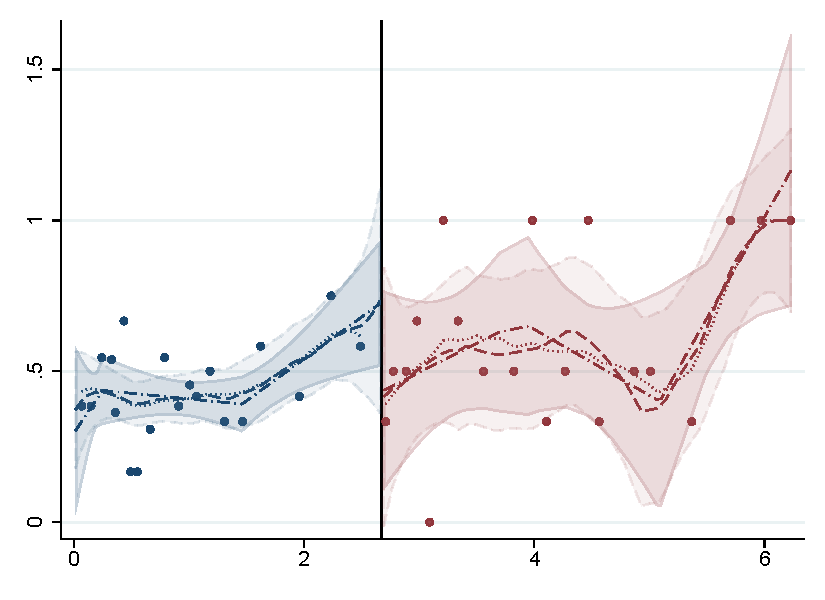
\includegraphics[width=\textwidth]{Figuras/rdplot_conflicto_arreglado_3_4_1.pdf}
    \end{subfigure}
\begin{subfigure}{0.31\textwidth}
\caption{(II \& III) vs (I \& IV)	(Tenure)}
        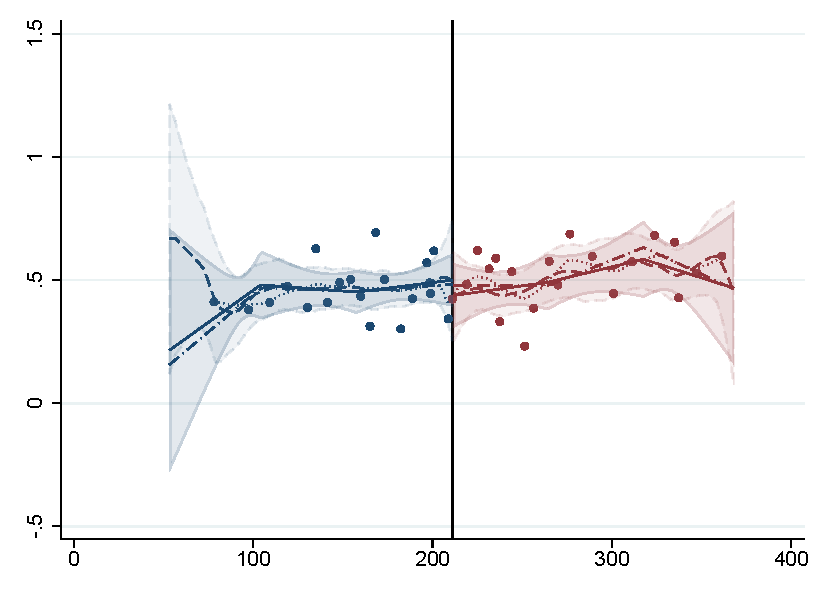
\includegraphics[width=\textwidth]{Figuras/rdplot_conflicto_arreglado_12_34_1.pdf}
    \end{subfigure}
    \begin{subfigure}{0.31\textwidth}
\caption{III vs II (Daily wage)}
        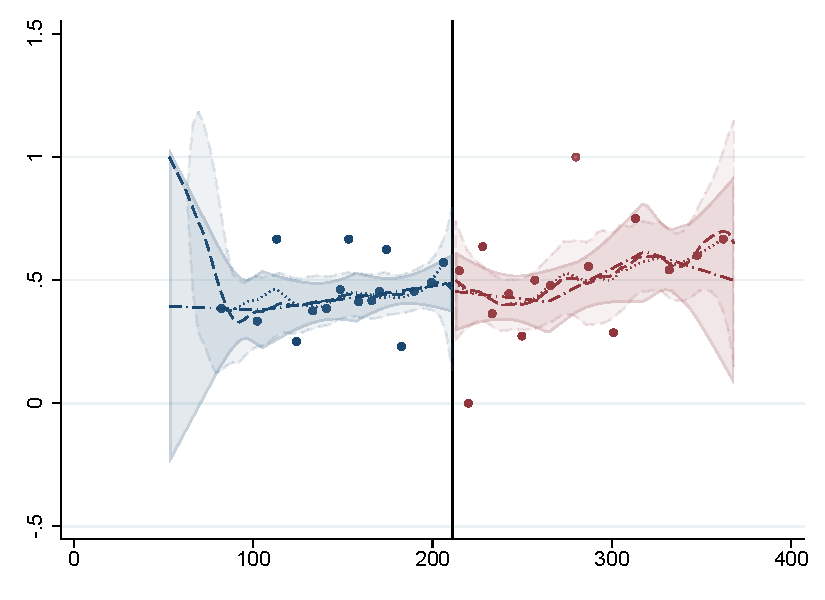
\includegraphics[width=\textwidth]{Figuras/rdplot_conflicto_arreglado_2_3_1.pdf}
    \end{subfigure}        
    \begin{subfigure}{0.31\textwidth}
\caption{IV vs I (Daily wage)}
        \includegraphics[width=\textwidth]{Figuras/rdplot_conflicto_arreglado_1_4_1.pdf}
    \end{subfigure}    
    \begin{subfigure}{0.31\textwidth}
\caption{(III \& IV) vs (I \& II) (Daily wage)}
        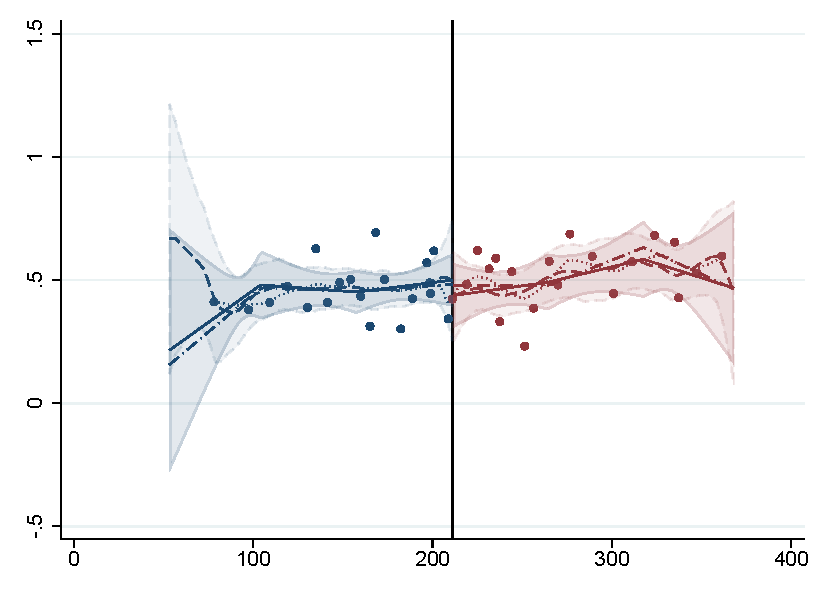
\includegraphics[width=\textwidth]{Figuras/rdplot_conflicto_arreglado_12_34_1.pdf}
    \end{subfigure}       
\begin{subfigure}{0.31\textwidth}
\caption{II vs IV (Tenure \& Daily wage)}
        \includegraphics[width=\textwidth]{Figuras/rdplot_conflicto_arreglado_2_4_1.pdf}
    \end{subfigure}
    \begin{subfigure}{0.31\textwidth}
\caption{III vs I (Tenure \& Daily wage)}
        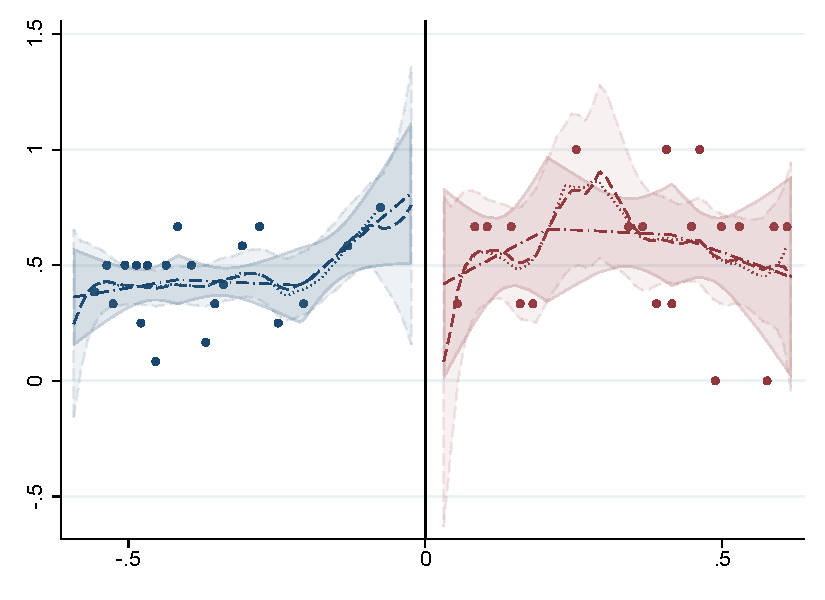
\includegraphics[width=\textwidth]{Figuras/rdplot_conflicto_arreglado_1_3_1.pdf}
    \end{subfigure}        
  \end{center}
  
    \scriptsize Regression discontinuity plots using 1) local polynomial smoothing 2) B-splines. \textcolor{yellow}{Me falta ajustar cosas de inferencia cuando uso los splines.}
%\textit{Scripts: }  \texttt{plot\_rd\_control.do}
\end{figure}




\begin{figure}[H]
     \caption{Estimation for artificial cutoffs (Calculator treatment)}
    \label{placebo_cutoff_t2}
\begin{center}
\begin{subfigure}{0.475\textwidth}
\caption{II vs I (Tenure)}
        \includegraphics[width=\textwidth]{Figuras/placebo_cut_1_2_2.pdf}
    \end{subfigure}
    \begin{subfigure}{0.475\textwidth}
\caption{III vs IV (Tenure)}
        \includegraphics[width=\textwidth]{Figuras/placebo_cut_3_4_2.pdf}
    \end{subfigure}
\begin{subfigure}{0.475\textwidth}
\caption{(II \& III) vs (I \& IV)	(Tenure)}
        \includegraphics[width=\textwidth]{Figuras/placebo_cut_23_14_2.pdf}
    \end{subfigure}
    \begin{subfigure}{0.475\textwidth}
\caption{III vs II (Daily wage)}
        \includegraphics[width=\textwidth]{Figuras/placebo_cut_2_3_2.pdf}
    \end{subfigure}        
    \begin{subfigure}{0.475\textwidth}
\caption{IV vs I (Daily wage)}
        \includegraphics[width=\textwidth]{Figuras/placebo_cut_1_4_2.pdf}
    \end{subfigure}    
    \begin{subfigure}{0.475\textwidth}
\caption{(III \& IV) vs (I \& II) (Daily wage)}
        \includegraphics[width=\textwidth]{Figuras/placebo_cut_12_34_2.pdf}
    \end{subfigure}       
      
  \end{center}
  
    \scriptsize 
%\textit{Scripts: }  \texttt{placebo\_cutoff.do}
\end{figure}






\begin{figure}[H]
     \caption{Estimation for artificial cutoffs (Calculator treatment)}
    \label{placebo_cutoff_t2}
\begin{center}
\begin{subfigure}{0.475\textwidth}
\caption{II vs I (Tenure)}
        \includegraphics[width=\textwidth]{Figuras/placebo_cut_1_2_2.pdf}
    \end{subfigure}
    \begin{subfigure}{0.475\textwidth}
\caption{III vs IV (Tenure)}
        \includegraphics[width=\textwidth]{Figuras/placebo_cut_3_4_2.pdf}
    \end{subfigure}
\begin{subfigure}{0.475\textwidth}
\caption{(II \& III) vs (I \& IV)	(Tenure)}
        \includegraphics[width=\textwidth]{Figuras/placebo_cut_23_14_2.pdf}
    \end{subfigure}
    \begin{subfigure}{0.475\textwidth}
\caption{III vs II (Daily wage)}
        \includegraphics[width=\textwidth]{Figuras/placebo_cut_2_3_2.pdf}
    \end{subfigure}        
    \begin{subfigure}{0.475\textwidth}
\caption{IV vs I (Daily wage)}
        \includegraphics[width=\textwidth]{Figuras/placebo_cut_1_4_2.pdf}
    \end{subfigure}    
    \begin{subfigure}{0.475\textwidth}
\caption{(III \& IV) vs (I \& II) (Daily wage)}
        \includegraphics[width=\textwidth]{Figuras/placebo_cut_12_34_2.pdf}
    \end{subfigure}       
      
  \end{center}
  
    \scriptsize 
%\textit{Scripts: }  \texttt{placebo\_cutoff.do}
\end{figure}

%__________________________________________________________________________
%__________________________________________________________________________
%__________________________________________________________________________
%__________________________________________________________________________


\begin{figure}[H]
     \caption{Estimation for artificial cutoffs (Calculator treatment)}
    \label{placebo_cutoff_t2}
\begin{center}
\begin{subfigure}{0.475\textwidth}
\caption{II vs I (Tenure)}
        \includegraphics[width=\textwidth]{Figuras/placebo_cut_1_2_2.pdf}
    \end{subfigure}
    \begin{subfigure}{0.475\textwidth}
\caption{III vs IV (Tenure)}
        \includegraphics[width=\textwidth]{Figuras/placebo_cut_3_4_2.pdf}
    \end{subfigure}
\begin{subfigure}{0.475\textwidth}
\caption{(II \& III) vs (I \& IV)	(Tenure)}
        \includegraphics[width=\textwidth]{Figuras/placebo_cut_23_14_2.pdf}
    \end{subfigure}
    \begin{subfigure}{0.475\textwidth}
\caption{III vs II (Daily wage)}
        \includegraphics[width=\textwidth]{Figuras/placebo_cut_2_3_2.pdf}
    \end{subfigure}        
    \begin{subfigure}{0.475\textwidth}
\caption{IV vs I (Daily wage)}
        \includegraphics[width=\textwidth]{Figuras/placebo_cut_1_4_2.pdf}
    \end{subfigure}    
    \begin{subfigure}{0.475\textwidth}
\caption{(III \& IV) vs (I \& II) (Daily wage)}
        \includegraphics[width=\textwidth]{Figuras/placebo_cut_12_34_2.pdf}
    \end{subfigure}       
      
  \end{center}
  
    \scriptsize 
%\textit{Scripts: }  \texttt{placebo\_cutoff.do}
\end{figure}


\clearpage
\bibliographystyle{authordate1}
%\bibliographystyle{amsalpha}
%\bibliographystyle{AER}

\bibliography{References}
